\documentclass[a4paper]{article}
\usepackage[english]{babel}
\usepackage[utf8]{inputenc}
\usepackage{textcomp}
\usepackage{amsmath}
\usepackage{gensymb}
\usepackage{physics}
\usepackage{graphicx}
\usepackage[colorinlistoftodos]{todonotes}
\usepackage{xcolor}
\usepackage{array}
\usepackage{tabularx}
\usepackage{tikz}
\usepackage{pgfplots}
\usepackage{framed}
\usepackage{xfrac}
\usepackage[most]{tcolorbox}
\usepackage{fix-cm}
\usepackage{cancel}
\usepackage[margin=0.5in]{geometry}
\usetikzlibrary{quotes,angles}
\usetikzlibrary{decorations.pathreplacing}
\usetikzlibrary{calc}
\usepgfplotslibrary{fillbetween}

\let\phi\varphi
\let\bf\textbf
\colorlet{shadecolor}{orange!15}
\pgfplotsset{compat=1.18}
\newcommand\der[2]{\frac{d #1}{d #2}}
\newcommand\Deltat{\Delta t}
\newcommand\rads{\text{ rad\;s}^{-1}}
\newcommand\radss{\text{ rad\;s}^{-2}}
\newcommand\rad{\text{ rad}}
\newcommand\s{\text{ s}}
\newcommand\m{\text{ m}}
\newcommand\km{\text{ km}}
\newcommand\J{\text{ J}}
\newcommand\Nm{\text{ Nm}}
\newcommand\ms{\text{ ms}^{-1}}
\newcommand\mss{\text{ ms}^{-2}}
\newcommand\kg{\text{ kg}}
\newcommand\kgms{\text{ kg\;ms}^{-1}}
\newcommand\kgmm{\text{ kg\;m}^{2}}
\newcommand\kgmms{\text{ kg\;m}^2\text{s}^{-1}}
\newcommand{\AxisRotator}[1][rotate=0]{%
    \tikz [x=0.25cm,y=0.60cm,line width=.2ex,-stealth,#1] \draw (0,0) arc (-150:150:1 and 1);%
}
\def\centerarc[#1](#2)(#3:#4:#5){\draw[#1] ($(#2)+({#5*cos(#3)},{#5*sin(#3)})$) arc (#3:#4:#5)}
% Syntax: \centerarc[draw options] (center) (initial angle:final angle:radius);

\title{Angular Momentum}
\author{OpenStax University Physics Vol. 1}
\date{}

\begin{document}
\setcounter{section}{11}
\maketitle
\subsection{Rolling Motion}
Rolling motion is the common combinatipno of rotational and translational motion seen every day, such as wheels moving on a car along a highway or wheels on a plane landing on a runway.\vspace{2mm}\\
\bf{Rolling Motion Without Slipping}\vspace{2mm}\\
Rolling motion without slipping has been observed since the invention of the wheel. For example, consider the interaction of a car's tires and the surface of the road. If the driver floors the accelerator such that the tires spin without moving the car, there must be kinetic friction between the wheels and the surface of the road. If the driver depresses the accelerator slowly causing the car to move forward, then the tires roll without slipping. In fact the bottom of the wheel is at rest with respect to the ground, indicating there must be static friction between the tires and the road surface.\vspace{1mm}\\
To analyze rolling without slipping, we first derive the linear variables of velocity and acceleration of the center of mass of the wheel in terms of the angular variables that describe the wheel's motion, shown below.

\begin{center}
    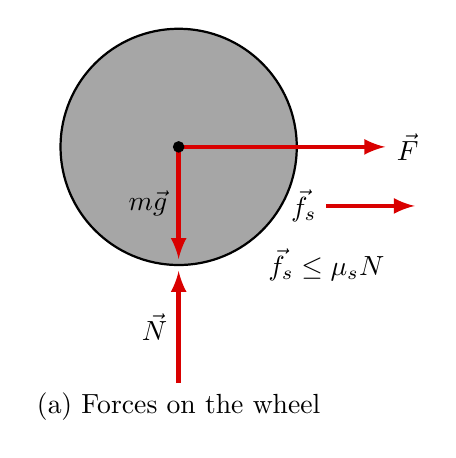
\begin{tikzpicture}[scale=1.5]
        \filldraw[black!35] (0,0) circle (1);
        \draw[black,thick] (0,0) circle (1);

        \draw[->,ultra thick,-latex,black!15!red] (0,0)--node[left,text=black]{$m\vec{g}$}(0,-0.95);
        \draw[->,ultra thick,-latex,black!15!red] (0,-2)--node[left,text=black]{$\vec{N}$}(0,-1.05);
        \draw[->,ultra thick,-latex,black!15!red] (0,0)--(1.75,0) node[right,text=black]{$\vec{F}$};
        \draw[->,ultra thick,-latex,black!15!red] (1.25,-0.5)--(2,-0.5);
        \node[left] at (1.25,-0.5){$\vec{f}_s$};
        \node at (1.25,-1){$\vec{f}_s \leq \mu_sN$};

        \filldraw[black] (0,0) circle  (1.25pt);
        \node at (0,-2.2){(a) Forces on the wheel};
    \end{tikzpicture}
    \hspace{5mm}
    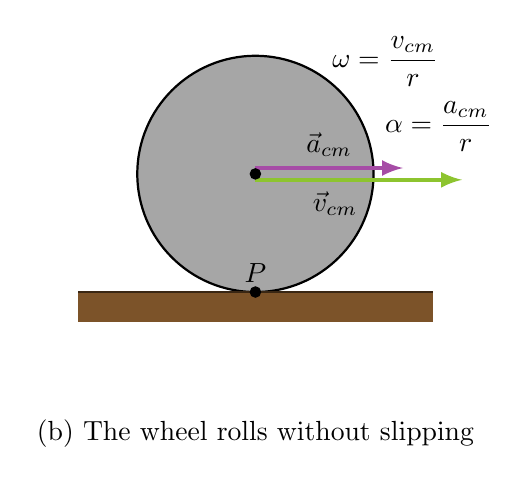
\begin{tikzpicture}[scale=1.5]
        \filldraw[black!35] (0,0) circle (1);
        \draw[black,thick] (0,0) circle (1);

        \draw[->,ultra thick,-latex,black!15!yellow!60!green] (0,-0.05)--node[below,text=black,xshift=-3mm]{$\vec{v}_{cm}$} (1.75,-0.05);
        \draw[->,ultra thick,-latex,white!30!violet] (0,0.05)--node[above,text=black]{$\vec{a}_{cm}$} (1.25,0.05);
        \filldraw[black!35!brown] (-1.5,-1) rectangle (1.5,-1.25);
        \draw[line width=0.5pt,draw=black!70!brown] (-1.5,-1)--(1.5,-1);

        \filldraw[black] (0,-1) circle (1.25pt) node[above]{$P$};
        \filldraw[black] (0,0) circle (1.25pt);
        \centerarc[<-,very thick,latex-,black](0,0)(150:225:1.25);

        \node at (1.1,0.95){$\displaystyle \omega = \frac{v_{cm}}{r}$};
        \node at (1.55,0.4){$\displaystyle \alpha = \frac{a_{cm}}{r}$};
        \node at (0,-2.2){(b) The wheel rolls without slipping};
    \end{tikzpicture}
    \hspace{5mm}
    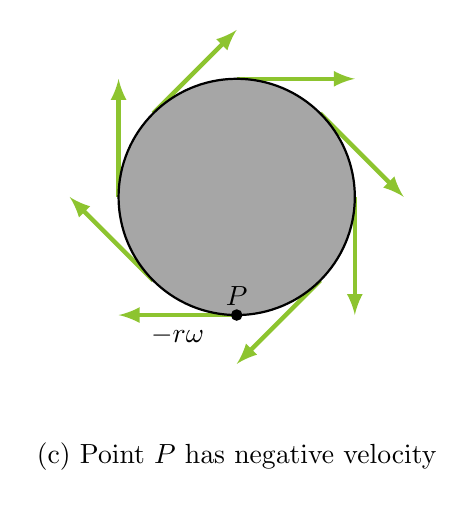
\begin{tikzpicture}[scale=1.5]
        \draw (0,1) coordinate (a);
        \draw (1,0) coordinate (b);
        \draw (0,-1) coordinate (c);
        \draw (-1,0) coordinate (d);
        \draw ({cos(45)},{sin(45)}) coordinate (e);
        \draw ({cos(45)},{-sin(45)}) coordinate (f);
        \draw ({-cos(45)},{-sin(45)}) coordinate (g);
        \draw ({-cos(45)},{sin(45)}) coordinate (h);

        \draw[->,ultra thick,-latex,black!15!yellow!60!green] (a)--([turn]-90:1);
        \draw[->,ultra thick,-latex,black!15!yellow!60!green] (b)--([turn]-90:1);
        \draw[->,ultra thick,-latex,black!15!yellow!60!green] (c)-- node[below,text=black]{$-r\omega$} ([turn]-90:1);
        \draw[->,ultra thick,-latex,black!15!yellow!60!green] (d)--([turn]-90:1);
        \draw[->,ultra thick,-latex,black!15!yellow!60!green] (e)--([turn]-90:1);
        \draw[->,ultra thick,-latex,black!15!yellow!60!green] (f)--([turn]-90:1);
        \draw[->,ultra thick,-latex,black!15!yellow!60!green] (g)--([turn]-90:1);
        \draw[->,ultra thick,-latex,black!15!yellow!60!green] (h)--([turn]-90:1);

        \filldraw[black!35] (0,0) circle (1);
        \draw[black,thick] (0,0) circle (1);
        \filldraw[black] (0,-1) circle (1.25pt) node[above]{$P$};

        \node at (0,-2.2){(c) Point $P$ has negative velocity};
    \end{tikzpicture}
\end{center}
In (a), we see the force vectors involved in preventing the wheel from slipping. In (b), the point $P$ that touches the surface is at rest relative to the surface. Relative to the center of mass, point $P$ has velocity $-r\omega\hat{i}$, where $r$ is the radius of the wheel and $\omega$ is the wheel's angular velocity about its axis. Since the wheel is rolling, the velocity of $P$ with respect to the surface is its velocity with respect to the center of mass plus the velocity of the center of mass with respect to the surface:
\begin{align*}
    \vec{v}_P = -r\omega\hat{i} + v_{cm}\hat{i}
\end{align*}
Since the velocity of $P$ relative to the surface is zero, $v_P = 0$, this says that:
\begin{equation}
    v_{cm} = r\omega
\end{equation}
The velocity of the wheel's center of mass is its radius times the angular velocity about its axis. Differentiating the left side of the equation gives an expression for the linear acceleration of the center of mass, on the right side, $r$ is constant and since $\alpha = \der{\omega}{t}$:
\begin{equation}
    a_{cm} = r\alpha
\end{equation}
Further, the distance the wheel travels can be found in terms of angular variables. As the wheel rolls from point $A$ to point $B$, its outer surface maps onto the ground by exactly the distance traveled $d_{cm}$. The length of the outer surface that maps onto the ground is the arc length $r\theta$. Equating the two distances gives:
\begin{equation}
    d_{cm} =  r\theta
\end{equation}
\begin{center}
    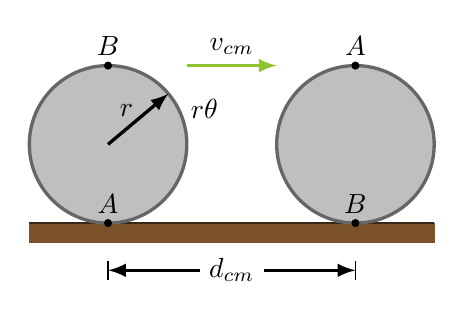
\begin{tikzpicture}[scale=1]
        %%% Ground %%%
        \filldraw[black!35!brown] (-1,-1) rectangle (4.1415,-1.25);
        \draw[line width=0.5pt,draw=black!70!brown] (-1,-1)--(4.1415,-1);

        %%% Circle 1 %%%
        \filldraw[black!25] (0,0) circle (1);
        \draw[black!60,very thick] (0,0) circle (1);
        \filldraw[black] (0,1) circle (1.25pt) node[above]{$B$};
        \filldraw[black] (0,-1) circle (1.25pt) node[above]{$A$};
        \draw[->,very thick,-latex] (0,0)--node[above,xshift=-1.5mm,yshift=-1mm]{$r$} ({cos(40)},{sin(40)});
        \node at ({1.3*cos(20)},{1.3*sin(20)}){$r\theta$};
        \centerarc[->,black!5!green!50!blue,very thick,latex-](0,0)(270:450:1);

        %%% Circle 2 %%%
        \filldraw[black!25] (3.1415,0) circle (1);
        \draw[black!60,very thick] (3.1415,0) circle (1);
        \filldraw[black] (3.1415,1) circle (1.25pt) node[above]{$A$};
        \filldraw[black] (3.1415,-1) circle (1.25pt) node[above]{$B$};
        \centerarc[-,black!5!green!50!blue,very thick](3.1415,0)(90:270:1);

        %%% d_{cm} %%%
        \draw[<->,very thick,latex-latex] (0,-1.6)--node[fill=white]{$d_{cm}$}(3.1415,-1.6);
        \draw[line width=0.5pt] (0,-1.48)--(0,-1.72);
        \draw[line width=0.5pt] (3.1415,-1.48)--(3.1415,-1.72);

        %%% v_{cm} %%%
        \draw[->,very thick,-latex,draw=black!15!yellow!60!green] (1,1)--node[above]{$v_{cm}$}(2.1415,1);
    \end{tikzpicture}
\end{center}

\begin{shaded}
    \underline{\bf{Example 11.1:} Rolling Down an Inclined Plane}
    \vspace{2mm}\\
    A solid cylinder rolls down an inclined plane without slipping, starting from rest. It has mass $m$ and radius $r$.
    \begin{enumerate}
        \item[(a)] What is its acceleration?
        \vspace{1mm}\\
        There is barely enough friction to keep the cylinder rolling without slipping. Since there is no slipping, the magnitude of the friction force is $f_s \leq \mu_sN$. Writing down Newton's laws in the $x$ and $y$ direction we have:
        \begin{align*}
            \sum F_x = ma_x\ \text{ and }\ \sum F_y = ma_y
        \end{align*}
        \begin{center}
            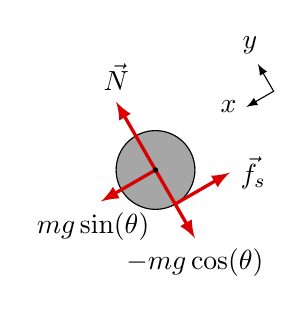
\begin{tikzpicture}
                \filldraw[black!35] (0,0) circle (0.5);
                \draw[black] (0,0) circle (0.5);

                \draw[->,very thick,draw=black!15!red,-latex] (0,0)--({-cos(60)},{sin(60)}) node[above]{$\vec{N}$};
                \draw[->,very thick,draw=black!15!red,-latex] (0,0)--({-0.8*cos(30)},{-0.8*sin(30)}) node[below,xshift=-1mm]{$mg\sin(\theta)$};
                \draw[->,very thick,draw=black!15!red,-latex] (0,0)--({cos(60)},{-sin(60)}) node[below]{$-mg\cos(\theta)$};
                \draw[->,very thick,draw=black!15!red,-latex] ({0.5*cos(60)},{-0.5*sin(60)})--({0.5*cos(60) + 0.8*cos(30)},{-0.5*sin(60) + 0.8*sin(30)}) node[right]{$\vec{f}_s$};

                \filldraw (0,0) circle (0.75pt);

                \draw[->,latex-latex] ({1.5 - 0.4*cos(30)},{1 - 0.4*sin(30)})--(1.5,1)--({1.5 - 0.4*cos(60)},{1 + 0.4*sin(60)}) node[above,xshift=-1mm]{$y$};
                \node[left] at ({1.5 - 0.4*cos(30)},{1 - 0.4*sin(30)}){$x$};
            \end{tikzpicture}
        \end{center}
        Substituting in from the free-body diagram:
        \begin{align*}
            mg\sin(\theta) - f_s &= m(a_{cm})\\
            N - mg\cos(\theta) &= 0
        \end{align*}
        The linear acceleration can then be solved for the linear acceleration of the center of mass using the equation
        \begin{align*}
            a_{cm} = g\sin(\theta) - \frac{f_s}{m}.
        \end{align*}
        However, it is useful to express the linear acceleration in terms of the moment of inertia, for this, use Newton's second law for rotation
        \begin{align*}
            \sum\tau_{cm} = I_{cm}\alpha
        \end{align*}
        The torques are calculated about the axis through the center of mass of the cylinder. The only nonzero torque is provided by the friction force:
        \begin{align*}
            f_sr = I_{cm}\alpha
        \end{align*}
        Finally, the linear acceleration is related to the angular acceleration by $a_{cm,x} = r\alpha$. These equations can be used to solve for $a_{cm}, \alpha,$ and $f_s$ in terms of the moment of inertia. $a_{cm}$ is rewritten in terms of the vertical component of gravity and the friction force, and the following substitutions are made:
        \begin{align*}
            f_s = \frac{I_{cm}\alpha}{r} = \frac{I_{cm}a_cm}{r^2}
        \end{align*}
        Substituting this in for $f_s$ in the equation above, gives:
        \begin{align*}
            a_{cm} &= g\sin(\theta) - \frac{I_{cm}a_{cm}}{mr^2}\\
            &= \frac{mg\sin(\theta)}{m + (\sfrac{I_{cm}}{r^2})}
        \end{align*}
        Therefore:
        \begin{align*}
            \alpha = \frac{a_{cm}}{r} = \frac{2}{3r}g\sin(\theta)
        \end{align*}
        \item[(b)] What condition must the coefficient of static friction $\mu_s$ satisfy so the cylinder does not slip?\vspace{2mm}\\
        Because slipping does not occur, $f_s \leq \mu_sN$. Solving for the friction force $f_s$,
        \begin{align*}
            f_s = I_{cm}\frac{\alpha}{r} = I_{cm}\frac{a_{cm}}{r^2} = \frac{I_{cm}}{r^2}\bigg(\frac{mg\sin(\theta)}{m + (\sfrac{I_{cm}}{r^2})}\bigg) = \frac{mgI_{cm}\sin(\theta)}{mr^2 + I_{cm}}
        \end{align*}
        Substituting in the condition for no slipping and noting that $N = mg\cos(\theta)$, gives
        \begin{align*}
            \frac{mgI_{cm}\sin(\theta)}{mr^2 + I_{cm}} \leq \mu_smg\cos(\theta)\ \text{ or }\ \mu_s \geq \frac{\tan(\theta)}{1 + (\sfrac{mr^2}{I_{cm}})}
        \end{align*}
        For the solid cylinder this becomes:
        \begin{align*}
            \mu_s \geq \frac{\tan(\theta)}{1 + (\sfrac{2mr^2}{mr^2})} = \frac{1}{3}\tan(\theta)
        \end{align*}
    \end{enumerate}
\end{shaded}
\newpage\noindent
It is worthwile to repeat the equation derived in the example for the acceleration of an object rolling without slipping:
\begin{equation}
    a_{cm} = \frac{mg\sin(\theta)}{1 + (\sfrac{I_{cm}}{r^2})}
\end{equation}
This equation is very useful for solving problems involving rolling without slipping. Note that the acceleration is less thana that of an object sliding down a frictionless plane with no rotation. The acceleration will also be different for two rotating objects with different rotational inertias.
\vspace{2mm}\\
\bf{Rolling Motion With Slipping}
\vspace{2mm}\\
In the case of rolling motion with slipping, we must use the coefficient of kinetic friction, which gives rise to the kinetic friction force since static friction is not present. In the case of slipping, $v_{cm} - r\omega \neq 0$, because the point $P$ on the wheel is not at rest on the surface, and $v_P \neq 0$. In this scenerio, $\omega \neq \frac{v_{cm}}{r}$ and $\alpha \neq \frac{a_{cm}}{r}$
\begin{center}
    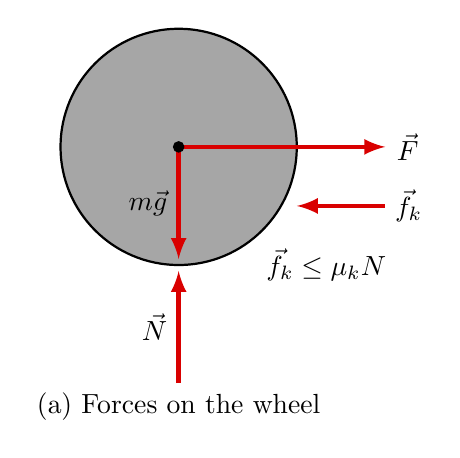
\begin{tikzpicture}[scale=1.5]
        \filldraw[black!35] (0,0) circle (1);
        \draw[black,thick] (0,0) circle (1);

        \draw[->,ultra thick,-latex,black!15!red] (0,0)--node[left,text=black]{$m\vec{g}$}(0,-0.95);
        \draw[->,ultra thick,-latex,black!15!red] (0,-2)--node[left,text=black]{$\vec{N}$}(0,-1.05);
        \draw[->,ultra thick,-latex,black!15!red] (0,0)--(1.75,0) node[right,text=black]{$\vec{F}$};
        \draw[->,ultra thick,latex-,black!15!red] (1,-0.5)--(1.75,-0.5);
        \node[right] at (1.75,-0.5){$\vec{f}_k$};
        \node at (1.25,-1){$\vec{f}_k \leq \mu_kN$};

        \filldraw[black] (0,0) circle  (1.25pt);
        \node at (0,-2.2){(a) Forces on the wheel};
    \end{tikzpicture}
    \hspace{5mm}
    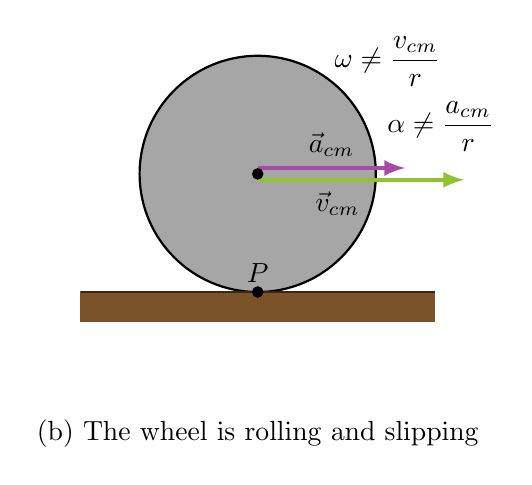
\begin{tikzpicture}[scale=1.5]
        \filldraw[black!35] (0,0) circle (1);
        \draw[black,thick] (0,0) circle (1);

        \draw[->,ultra thick,-latex,black!15!yellow!60!green] (0,-0.05)--node[below,text=black,xshift=-3mm]{$\vec{v}_{cm}$} (1.75,-0.05);
        \draw[->,ultra thick,-latex,white!30!violet] (0,0.05)--node[above,text=black]{$\vec{a}_{cm}$} (1.25,0.05);
        \filldraw[black!35!brown] (-1.5,-1) rectangle (1.5,-1.25);
        \draw[line width=0.5pt,draw=black!70!brown] (-1.5,-1)--(1.5,-1);

        \filldraw[black] (0,-1) circle (1.25pt) node[above]{$P$};
        \filldraw[black] (0,0) circle (1.25pt);
        \centerarc[<-,very thick,latex-,black](0,0)(150:225:1.25);

        \node at (1.1,0.95){$\displaystyle \omega \neq \frac{v_{cm}}{r}$};
        \node at (1.55,0.4){$\displaystyle \alpha \neq \frac{a_{cm}}{r}$};
        \node at (0,-2.2){(b) The wheel is rolling and slipping};
    \end{tikzpicture}
\end{center}

\begin{shaded}
    \underline{\bf{Example 11.2:} Rolling Down an Inclined Plane With Slipping}
    \vspace{2mm}\\
    A solid cylinder rolls down an inclined plane from rest and undergoes slipping. It has a mass $m$ and a radius $r$.\vspace{1mm}\\
    Draw a skech and free-body diagram showing the forces involved. The free-body diagram is similar to the no-slipping case except for the friction force, which is kinetic rather than static. Use Newton's second law to solve for the acceleration in the $x$ direction, and use Newton's second law of rotation to solve for the angular acceleration
    \begin{center}
        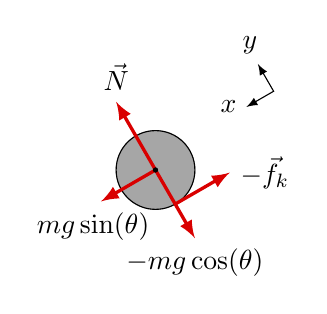
\begin{tikzpicture}
            \filldraw[black!35] (0,0) circle (0.5);
            \draw[black] (0,0) circle (0.5);

            \draw[->,very thick,draw=black!15!red,-latex] (0,0)--({-cos(60)},{sin(60)}) node[above]{$\vec{N}$};
            \draw[->,very thick,draw=black!15!red,-latex] (0,0)--({-0.8*cos(30)},{-0.8*sin(30)}) node[below,xshift=-1mm]{$mg\sin(\theta)$};
            \draw[->,very thick,draw=black!15!red,-latex] (0,0)--({cos(60)},{-sin(60)}) node[below]{$-mg\cos(\theta)$};
            \draw[->,very thick,draw=black!15!red,-latex] ({0.5*cos(60)},{-0.5*sin(60)})--({0.5*cos(60) + 0.8*cos(30)},{-0.5*sin(60) + 0.8*sin(30)}) node[right]{$-\vec{f}_k$};

            \filldraw (0,0) circle (0.75pt);

            \draw[->,latex-latex] ({1.5 - 0.4*cos(30)},{1 - 0.4*sin(30)})--(1.5,1)--({1.5 - 0.4*cos(60)},{1 + 0.4*sin(60)}) node[above,xshift=-1mm]{$y$};
            \node[left] at ({1.5 - 0.4*cos(30)},{1 - 0.4*sin(30)}){$x$};
        \end{tikzpicture}
    \end{center}
    \begin{enumerate}
        \item[(a)] What is its linear acceleration?\\
        The sum of the forces in the $y$ direction is zero, so the friction force is $f_k = \mu_kN = \mu_k$\\
        Newton's second law in the $x$ direction becomes:
        \begin{align*}
            \sum F_x &= ma_x\\
            mg\sin(\theta) - \mu_kmg&\cos(\theta) = ma_{cm,x}
        \end{align*}
        Which rearranges to 
        \begin{align*}
            a_{cm,x} = g\big(sin(\theta) - \mu_k\cos(\theta)\big)
        \end{align*}
        \item[(b)] What is its angular acceleration about an axis through the center of mass?\\
        The friction force provides the only torque about the axis through the center of mass, so Newton's second law of rotation becomes:
        \begin{align*}
            \sum\tau_{cm} &= I_{cm}\alpha\\
            f_kr &= I_{cm}\alpha = \frac{1}{2}mr^2\alpha
        \end{align*}
        Solving or $\alpha$ gives:
        \begin{align*}
            \alpha = \frac{2f_k}{mr} = \frac{2\mu_kg\cos(\theta)}{r}
        \end{align*}
    \end{enumerate}
\end{shaded}
\newpage

\noindent\bf{Conservation of Mechanical Energy in Rolling Motion}
\vspace{2mm}\\
Any rolling object carries rotational kinetic energy, as well as translational kinetic energy and potential energy if the system requires. Including the gravitational potential energy, the total mechanical energy of a rolling object is:
\begin{align*}
    E_T = \frac{1}{2}mv^2_{cm} + \frac{1}{2}I_{cm}\omega^2 + mgh
\end{align*}
In the absence of any nonconservative forces that would take energy out of the system in the form of heat, the total energy of a rolling object without slipping is conserved and is constant throughout the motion. In a rolling object that is slipping, energy is not conserved, the production of heat is the result of kinetic friction and a rolling object encountering air resistance.\vspace{1mm}\\
You may ask why a rolling object that is not slipping conserves energy, since the static friction force is nonconservative. The answer relates to the figure where point $P$ is shown in contact with the surface and at rest relative to the surface. Therefore the infinitesimal displacement $d\vec{r}$ with respect to the surface is zero and the incremental work done by the static friction is zero.
\begin{shaded}
    \underline{\bf{Example 11.3} Curiosity Rover}
    \vspace{2mm}\\
    The Curiosity rover was deployed on Mars on August 6, 2012. The wheels of the rover have a radius of 25 cm. Suppose astronauts arrive on Mars in the year 2050 and find the now inoperative Curiosity on the side of a basin. While they are dismantling the rover, an astronaut accidentially loses grip of one of the wheels, which rolls without slipping down into the bottom of the basin 25 meters below. If the wheel has a mass of 5 kg, what is its velocity at the bottom of the basin?\vspace{1mm}\\
    To solve the problem, use conservation of mechanical energy. At the top of the hill, the wheel is at rest and has only potential energy, at the bottom is has rotational and translational kinetic energy which must be equal to the initial potential energy. Since the wheel rolls without slipping, $v_{cm} = r\omega$.
    \vspace{1mm}\\
    The energy at the top is equal to the energy at the bottom:
    \begin{align*}
        mgh = \frac{1}{2}mv_{cm}^2 + \frac{1}{2}I_{cm}\omega^2
    \end{align*}
    The known quantities are $I_{cm} = mr^2$, $r = 0.25$ m, and $f = 25.0$ m. Rewriting the energy conservation equation, to solve for $v_{cm}$, eliminating $\omega$ using $\omega = \frac{v_{cm}}{r^2}$ gives:
    \begin{align*}
        mgh &= \frac{1}{2}mv_{cm}^2 + \frac{1}{2}mr^2\frac{v_{cm}^2}{r^2}\\
        gh &= \frac{1}{2}v_{cm}^2 + \frac{1}{2}v_{cm}^2\\
        v_{cm} &= \sqrt{gh}
    \end{align*}
    On Mars, the acceleration of gravity is 3.71$mss$, which gives the magnitude of velocity at the bottom of the basin as:
    \begin{align*}
        v_{cm} = \sqrt{\big(3.71\mss\big)(25.0\m)} = 9.63\ms
    \end{align*}
\end{shaded}
\newpage

\subsection{Angular Momentum}
\bf{Angular Momentum of a Single Particle}
\vspace{2mm}\\
The figure shows a particle at a position $\vec{r}$ with linear momentum $\vec{p} = m\vec{v}$ with respect to the origin. Even if the particle is not rotating about the origin, we can still define an angular momentum in terms of the position vector and the linear momentum. \vspace{1mm}\\
The angular momentum $\vec{l}$ is defined as the cross product of $\vec{r}$ and $\vec{p}$, and is perpendicular to the plane containing $\vec{r}$ and $\vec{p}$:
\begin{equation}
    \vec{l} = \vec{r} \times \vec{p}
\end{equation}
\begin{center}
    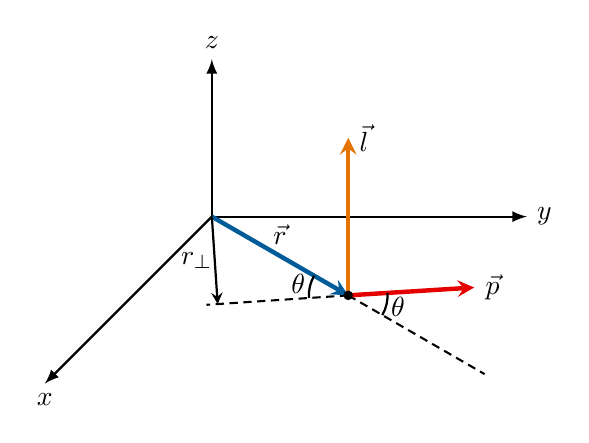
\begin{tikzpicture}[scale=2]
        \draw (0,0) coordinate (O) node[left]{};
        \draw ({cos(30)},{-sin(30)}) coordinate (P) node[below]{};
        \draw ({cos(30) + 0.8},{-sin(30) + 0.05}) coordinate (F);
        \draw ({cos(30) - 0.9},{-sin(30) - 0.06}) coordinate (F2);
        \draw ({cos(30) - 0.7},{-sin(30) - 0.04}) coordinate (F3);
        \draw ({2*cos(30)},{-2*sin(30)}) coordinate (P2);
        
        \draw[line width=0.75pt,densely dashed] (P)--({2*cos(30)},{-2*sin(30)});
        \draw[line width=0.75pt,densely dashed] (P)--(F2);
        \draw[->,thick,-latex] (0,0)--(0,1) node[above]{$z$};
        \draw[->,thick,-latex] (0,0)--(2,0) node[right]{$y$};
        \draw[->,thick,-latex] (0,0)--({-1.5*cos(45)},{-1.5*sin(45)}) node[below]{$x$};

        \draw[->,ultra thick,-stealth,draw=black!10!green!40!blue] (O)--node[above]{$\vec{r}$}(P);
        \draw[->,ultra thick,-stealth,draw=black!10!orange] (P)--({cos(30)},0.5) node[right]{$\vec{l}$};
        \draw[->,ultra thick,-stealth,draw=black!10!red] (P)--(F) node[right]{$\vec{p}$};

        \draw[->,thick,-stealth] (O)--node[left,xshift=1mm]{$r_{\perp}$} ($(P)!(O)!(F2)$);
        \draw pic["$\theta$",draw=black,-,thick,angle eccentricity=1.3,angle radius=5mm]{angle=O--P--F2};
        \draw pic["$\theta$",draw=black,-,thick,angle eccentricity=1.3,angle radius=5mm]{angle=P2--P--F};

        \filldraw (P) circle (0.75pt);
    \end{tikzpicture}
\end{center}
The intent of choosing the direction of the angular momentum to be perpendicular to the plane containing $\vec{r}$ and $\vec{p}$ is similar to choosing the direction of torque to be perpendicular to the plane of $\vec{r}$ and $\vec{F}$. The magnitude of the angular momentum is found from the definition of a cross product:
\begin{align*}
    l = rp\sin(\theta)
\end{align*}
Where $\theta$ is the angle between $\vec{r}$ and $\vec{p}$. The units of angular momentum are $\kgmms$. As with the definition of torque, we can define a lever arm $r_{\perp}$ that is the perpendicular distance from the momentum vector $\vec{p}$ to the origin, $r_{\perp} = r\sin(\theta)$. With this definition, the magnitude of angular acceleration becomes:
\begin{align*}
    l = r_{\perp}p = r_{\perp}mv
\end{align*}
The direction of $\vec{p}$ is such that it passes through the origin, then $\theta = 0$, and the angular momentum is zero because the lever arm is zero. In this respect, the magnitude of the angular momentum depends on the choice of origin. Taking the time derivative of the angular momentum gives an expression for the torque on the particle:
\begin{align*}
    \der{\vec{l}}{t} = \der{\vec{r}}{t} \times \vec{p} + \vec{r} \times \der{\vec{p}}{t} = \vec{v} \times m\vec{v} + \vec{r} \times \der{\vec{p}}{t} = \vec{r} \times \der{\vec{p}}{t}
\end{align*}
Here, the definition of $\vec{p}$ and the fact that a vector crossed into itself is zero is used. From Newton's second law, $\der{\vec{p}}{t} = \sum\vec{F}$, the net force acting on the particle, and the definition of the net torque we can write:
\begin{equation}
    \der{\vec{l}}{t} = \sum \vec{\tau}
\end{equation}
Note the similarity with the linear result of Newton's second law, $\der{\vec{p}}{t} = \sum\vec{F}$
\begin{shaded}
    \underline{\bf{Problem Solving Strategy:} Angular Momentum of a Particle}
    \begin{enumerate}
        \item Choose a coordinate system about which the angular momentum is to be calculated
        \item Write down the radius vector to the point particle in unit vector notation
        \item Write the linear momentum vector of the particle in unit vector notation
        \item Take the cross product $\vec{l} = \vec{r} \times \vec{p}$ and use the right-hand rule to establish the direction of the angular momentum vector
        \item See if there is a time dependence in the expression of the angular momentum vector. If there is, then a torque exists about the origin, use $\der{\vec{l}}{t} = \sum\vec{\tau}$ to calculate the torque. If there is no time dependence in the expression of angular momentum, then the net torque is zero
    \end{enumerate}
\end{shaded}
\newpage
\begin{shaded}
    \underline{\bf{Example 11.4:} Angular Momentum and Torque on a Meteor}
    \vspace{2mm}\\
    A meteor enters Earth's atmosphere and is observed by someone on the ground before it burns up in the atmosphere. The vector $\vec{r} = 25\km\hat{i} + 25\km\hat{j}$ gives the position of the metero with respect to the observer. At the instant the observer sees the meteor, it has a linear momentum of $15.0\kg(-2.0\km\s^{-1}\hat{j})$, and is accelerating at a constant $-2.0\mss\hat{j}$ along its path, which can be taken as a straight line.
    \begin{center}
        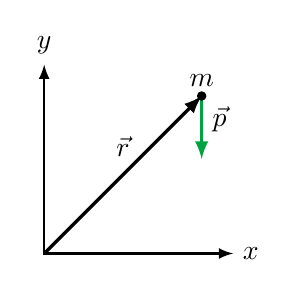
\begin{tikzpicture}[scale=2]
            \draw (1,1) coordinate (a);
            \draw[->,thick,latex-latex] (1.2,0)--(0,0)--(0,1.2) node[above]{$y$};
            \node[right] at (1.2,0){$x$};
            \draw[->,very thick,-latex] (0,0)--node[above,yshift=1mm]{$\vec{r}$}(a);
            \draw[->,very thick,-latex,draw=black!15!green!75!blue] (a)--node[right,yshift=1mm]{$\vec{p}$}(1,0.6);

            \filldraw (1,1) circle (0.75pt) node[above]{$m$};
        \end{tikzpicture}
    \end{center}
    The meteor is entering Earth's atmosphere at an angle of $90.0\degree$ below the horizontal, so the components of acceleration in the $x$ and $y$ directions are: $a_X = 0$ and $a_y = -2.0\mss$\\
    Write down the velocities using kinematic equations:
    \begin{align*}
        v_x = 0,\quad v_y = -2.0\cdot10^3\ms - (2.0\mss)t
    \end{align*}
    \begin{enumerate}
        \item[(a)] What is the angular momentum of the meteor about the origin?\\
        The angular momentum is:
        \begin{align*}
            \vec{l} &= \vec{r} \times \vec{p} = (25.0\km\hat{i} + 25.0\km\hat{j}) \times (15.0\kg)(0\hat{i} + v_y\hat{j})\\
            &= (15.0\kg)\big(25.0\km(v_y)\hat{k}\big)\\
            &= (15.0\kg)\big(2.50\cdot10^4\m(-2.0\cdot10^3\ms - (2.0\mss)t)\hat{k}\big)
        \end{align*}
        At $t = 0$, the angular momentum of the meteor about the origin is
        \begin{align*}
            \vec{l}_0 = (15.0\kg)\big(2.50\cdot10^4\m(-2.0\cdot10^3\ms)\hat{k}\big) = -7.50\cdot10^8\kgmms\hat{k}
        \end{align*}
        This is the instant that the observer sees the meteor
        \item[(b)] What is the torque on the meteor about the origin?\\
        To find the torque, take the time derivative of angular momentum. Taking the time derivative of $\vec{l}$ as a function of time, which is the second equation above, gives:
        \begin{align*}
            \der{\vec{l}}{t} = (15.0\kg)(2.50\cdot10^4\m)(2.0\mss)\hat{k}
        \end{align*}
        Then since $\der{\vec{l}}{t} = \sum\vec{\tau}$, we have
        \begin{align*}
            \sum\vec{\tau} = -7.5\cdot10^5\Nm\;\hat{k}
        \end{align*}
        As a check, note that the lever arm is the $x$ component of the vector $\vec{r}$ in the figure since it is perpendicular to the force acting on the meteor, which is along its path. By Newton's second law, the force is
        \begin{align*}
            \vec{F} = ma(-\hat{j}) = (15.0\kg)(2.0\mss)(-\hat{j}) = 30.0\text{ N}(-\hat{j})
        \end{align*}
        The lever arm is:
        \begin{align*}
            \vec{r}_{\perp} = 2.5\cdot10^4\m\;\hat{i}
        \end{align*}
        And thus the torque is:
        \begin{align*}
            \sum\vec{\tau} &= \vec{r}_{\perp}\times\vec{F}\\
            &= (2.5\cdot10^4\m\;\hat{i}) \times (-30\text{ N}\;\hat{j})\\
            &= 7.5\cdot10^5\Nm\;(-\hat{k})
        \end{align*}
        Since the meteor is accelerating downward towards Earth, its radius and velocity vector are changing. Therefore, since $\vec{l} = \vec{r} \times \vec{p}$, the angular momentum is changing as a function of time. The torque on the meteor about the origin however, is constant, because the lever arm $\vec{r}_{\perp}$ and the force on the meteor are constants.
    \end{enumerate}
\end{shaded}
\newpage
\noindent\bf{Angular Momentum of a System of Particles}
\vspace{2mm}\\
The angular momentum of a system of particles is important in many scientific disciplines, one being astronomy. Consider a spiral galaxy rotating, the individual stars can be treated as point particles, each of which has its own angular momentum. The vector sum of the individual angular momenta gives the total angular momentum of the galaxy.
\vspace{1mm}\\
The expression for the angular momentum of a single particle about a designated origin is $\vec{l} = \vec{r} \times \vec{p}$, where the vector $\vec{r}$ is from the origin to the particle and $\vec{p}$ is the particle's linear momentum. If we have a system of $N$ particles each with a position vector from the origin $\vec{r}_i$, and each having momentum $\vec{p}_i$, then the total angular momentum of the system of particles about the origin is the vector sum of the individual angular momenta about the origin, that is:
\begin{equation}
    \vec{L} = \vec{l}_1 + \vec{l}_2+ ... + \vec{l}_N
\end{equation}
Similarly, if particle $i$ is subject to a net torque $\vec{\tau}_i$ about the origin, then the net torque about the origin due to the system of particles can be found by differentiating equation 7:
\begin{align*}
    \der{\vec{L}}{t} = \sum_{i}\der{\vec{l}_i}{t} = \sum_{i}\vec{\tau}_i
\end{align*}
The sum of the individual torques produces a net external force on the system which we designate $\sum\vec{\tau}$, thus:
\begin{equation}
    \der{\vec{L}}{t} = \sum\vec{\tau}
\end{equation}
This states that the rate of change of the total angular momentum of a system is equal to the net external torque acting on the system when both quantities are measured with respect to a given origin. This can be applied to any system that has net angular momentum, including rigid bodies as discussed in the following section
\begin{shaded}
    \underline{\bf{Example 11.5:} Angular Momentum of Three Particles}
    \vspace{2mm}\\
    Referring to the figure below,
    \begin{center}
        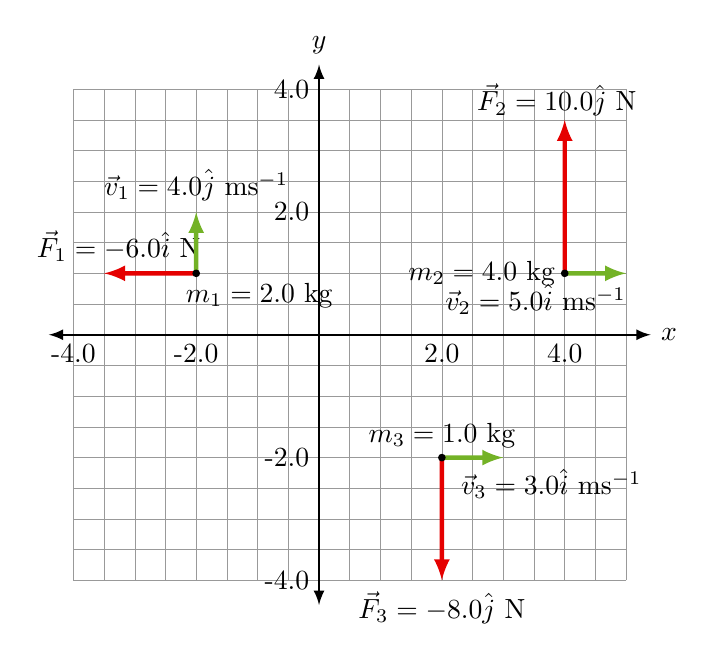
\begin{tikzpicture}[scale=0.78]
            %%% AXIS/GRID %%%
            \draw[step=0.5,very thin,gray!80] (-4,-4) grid (5,4);
            \draw[<->,thick,latex-latex] (-4.4,0)--(5.4,0) node[right]{$x$};
            \draw[<->,thick,latex-latex] (0,-4.4)--(0,4.4) node[above]{$y$};

            %%% COORDINATES %%%
            \draw (-2,1) coordinate (m1);
            \draw (4,1) coordinate (m2);
            \draw (2,-2) coordinate (m3);
            
            %%% TICKS %%%
            \node[below] at (-2,0){-2.0};
            \node[below] at (-4,0){-4.0};
            \node[below] at (2,0){2.0};
            \node[below] at (4,0){4.0};
            \node[left] at (0,-2){-2.0};
            \node[left] at (0,-4){-4.0};
            \node[left] at (0,2){2.0};
            \node[left] at (0,4){4.0};

            %%% FORCES %%%
            \draw[->,ultra thick,-latex,draw=black!10!red] (m1)--node[above,xshift=-4mm]{$\vec{F}_1 = -6.0\hat{i}\text{ N}$}(-3.5,1);
            \draw[->,ultra thick,-latex,draw=black!10!red] (m2)--(4,3.5) node[above,yshift=-1mm,xshift=-1mm]{$\vec{F}_2 = 10.0\hat{j}\text{ N}$};
            \draw[->,ultra thick,-latex,draw=black!10!red] (m3)--(2,-4) node[below]{$\vec{F}_3 = -8.0\hat{j}\text{ N}$};

            %%% VELOCITY %%%
            \draw[->,ultra thick,-latex,draw=brown!60!green] (m1)--(-2,2) node[above]{$\vec{v}_1 = 4.0\hat{j}\ms$}; 
            \draw[->,ultra thick,-latex,draw=brown!60!green] (m2)--(5,1) node[below,xshift=-1.15cm]{$\vec{v}_2 = 5.0\hat{i}\ms$};
            \draw[->,ultra thick,-latex,draw=brown!60!green] (m3)--node[below,xshift=1cm]{$\vec{v}_3 = 3.0\hat{i}\ms$}(3,-2);

            %%% POINTS %%%
            \filldraw (-2,1) circle (1.5pt) node[below,xshift=8mm]{$m_1 = 2.0\kg$}; % m1
            \filldraw (4,1) circle (1.5pt) node[left]{$m_2 = 4.0\kg$}; % m2
            \filldraw (2,-2) circle (1.5pt) node[above]{$m_3 = 1.0\kg$}; % m3
        \end{tikzpicture}
    \end{center}
    Known values: $\vec{r}_1 = -2.0\m\;\hat{i} + 1.0\m\;\hat{j},\ \vec{p}_1 = 2.0\kg(4.0\ms\;\hat{j}) = 8.0\kgms\;\hat{j}$ \\
    \hspace*{22.7mm} $\vec{r}_2 = 4.0\m\;\hat{i} + 1.0\m\;\hat{j},\ \vec{p}_2 = 4.0\kg(5.0\ms\;\hat{i}) = 20.0\kgms\;\hat{i}$\\
    \hspace*{22.7mm} $\vec{r}_3 = 2.0\m\;\hat{i} - 2.2\m\;\hat{j},\ \vec{p}_3 = 1.0\kg(3.0\ms\;\hat{i}) = 3.0\kgms$
    \begin{enumerate}
        \item[(a)] Determine the total angular momentum due to the three particles about the origin.\\
        For particle 1: $\vec{l}_1 = \vec{r}_1 \times \vec{p}_1 = -16\kgmms\;\hat{k}$\\
        For particle 2: $\vec{l}_2 = \vec{r}_2 \times \vec{p}_2 = -20.0\kgmms\;\hat{k}$\\
        For particle 3: $\vec{l}_3 = \vec{r}_3 \times \vec{p}_3 = 6.0\kgmms\;\hat{k}$
        \item[(b)] What is the rate of change of the angular momentum?
        The individual forces and lever arms are:
        \begin{align*}
            \vec{r}_{1,\perp} &= 1.0\m\;\hat{j},\ \vec{F}_1 = -6.0\text{ N}\hat{i},\ \vec{\tau}_1 = 6.0\Nm\;\hat{k}\\
            \vec{r}_{2,\perp} &= 4.0\m\;\hat{i},\ \vec{F}_2 = 10.0\text{ N}\hat{j},\ \vec{\tau}_1 = 40.0\Nm\;\hat{k}\\
            \vec{r}_{3,\perp} &= 2.0\m\;\hat{i},\ \vec{F}_3 = -8.0\text{ N}\hat{j},\ \vec{\tau}_1 = -16.0\Nm\;\hat{k}
        \end{align*}
        Therefore:
        \begin{align*}
            \sum_{i}\vec{\tau}_i = \vec{\tau}_1 + \vec{\tau}_2 + \vec{\tau}_3 = 30\Nm\;\hat{k}
        \end{align*}
    \end{enumerate}
\end{shaded}
\newpage

\noindent\bf{Angular Momentum of a Rigid Body}
\vspace{2mm}\\
To develop the angular momentum of a rigid body, we model a rigid body as being made up of small mass segments $\Delta m_i$. In the figure, a rigid body is constrained to rotate about the $z$ axis with angular velocity $\omega$. All mass segments that make up the rigid body undergo circular motion about the $z$ axis with the same angular velocity. Part (a) of the figure shows mass segment $\Delta m_i$ with position vector $\vec{r}_i$ from the origin and radius $R_i$ to the $z$ axis. The magnitude of its tangential velocity is $v_i = R_i\omega$. Because the vectors $\vec{v}_i$ and $\vec{r}_i$ are perpendicular to each other, the magnitude of the angular momentum of this mass segment it:
\begin{align*}
    l_i = r_i(\Delta mv_i)\sin(90\degree)
\end{align*}
\begin{center}
    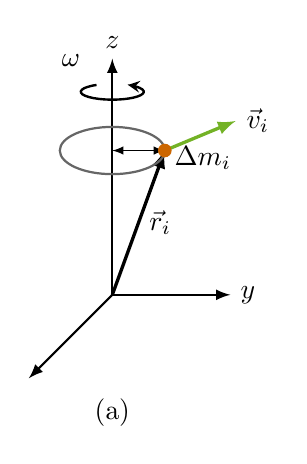
\begin{tikzpicture}[scale=1.5]
        \draw[<->,thick,latex-latex] (0,2)--(0,0)--(1,0) node[right]{$y$};
        \node[above] at (0,2){$z$};
        \draw[<->,thick,-latex] (0,0)--({-cos(45)},{-sin(45)});
        \draw[->,very thick,-latex] (0,0)--node[right]{$\vec{r}_i$}({1.3*cos(70)},{1.3*sin(70)}) coordinate (a);
        \draw[->,very thick,-latex,brown!60!green] (a)--({1.3*cos(70) + 0.6},{1.3*sin(70) + 0.25}) node[right,text=black]{$\vec{v}_i$};
        \draw[thick,black!60] (0,1.2216) ellipse (0.44462 and 0.2);
        \draw[<->,thin,latex-latex] ({1.3*cos(70)},{1.3*sin(70)})--(0,1.2216);
        \filldraw[black!20!orange] ({1.3*cos(70)},{1.3*sin(70)}) circle (1.5pt) node[right,yshift=-1mm,text=black]{$\Delta m_i$};
        \centerarc[->,-latex](0,1.2216)(165:195:0.6);
        \node[above] at (0,1.55){\AxisRotator[x=0.1cm,y=0.4cm,rotate=-90]};
        \node[above] at (-0.35,1.85){$\omega$};
        \node at (0,-1){(a)};
    \end{tikzpicture}
    \hspace{25mm}
    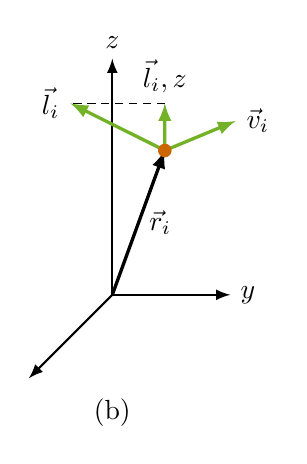
\begin{tikzpicture}[scale=1.5]
        \draw[<->,thick,latex-latex] (0,2)--(0,0)--(1,0) node[right]{$y$};
        \node[above] at (0,2){$z$};
        \draw[<->,thick,-latex] (0,0)--({-cos(45)},{-sin(45)});
        \draw[->,very thick,-latex] (0,0)--node[right]{$\vec{r}_i$}({1.3*cos(70)},{1.3*sin(70)}) coordinate (a);

        \draw[->,very thick,-latex,brown!60!green] (a)--({1.3*cos(70) + 0.6},{1.3*sin(70) + 0.25}) node[right,text=black]{$\vec{v}_i$};
        \draw[->,very thick,-latex,brown!60!green] (a)--({1.3*cos(70)},{1.3*sin(70) + 0.4}) coordinate (b) node[above,text=black]{$\vec{l}_i,z$};
        \draw[->,very thick,-latex,brown!60!green] (a)--({1.3*cos(70) - 0.8},{1.3*sin(70) + 0.4}) coordinate (c) node[left,text=black]{$\vec{l}_i$};
        \draw[line width=0.5pt,densely dashed] (b)--(c);
        \filldraw[black!20!orange] ({1.3*cos(70)},{1.3*sin(70)}) circle (1.5pt);
        \node at (0,-1){(b)};
    \end{tikzpicture}
\end{center}
Using the right-hand rule, the angular momentum vector points in the direction shown in part (b). The sum of the angular momenta of all the mass segments contains components both along and perpendicular to the axis of rotation. Every mass segment has a perpendicular component of the angular momentum that will be cancelled by the perpendicular component of an identical mass segment on the opposite side of the rigid body, because it is cylindrically symmetric. The component along the axis of rotation is the only component that gives a non-zero value when summed over all the mass segments. From part (b), the component of $\vec{l}_i$ along the axis of rotation is
\begin{align*}
    l_{i,z} &= l_i\sin(\theta_i) = (r_i\Delta m_iv_i)\sin(\theta_i)\\
    &= (r_i\sin(\theta_i))(\Delta m_iv_i) = R_i\Delta m_iv_i
\end{align*}
The net angular momentum of the rigid body along the axis of rotation is 
\begin{align*}
    L = \sum_{i}\vec{l}_{i,z} = \sum_{i}R_i\Delta m_iv_i = \sum_{i}R_i\Delta m_i(R_i\omega) = \omega\sum_{i}\Delta m_i(R_i)^2
\end{align*}
The summation $\sum\limits_{i}\Delta m_i(R_i)^2$ is simply the moment of inertia $I$ of the rigid body about the axis of rotation. For a thin hoop rotating about an axis perpendicular to the plane of the hoop, all the $R_i$'s are equal to $R$ so the summation reduces to $R^2\sum\limits_{i}\Delta m_i = mR^2$ which is the moment of inertia for a thin hoop. Thus, the magnitude of the angular momentum along the axis of rotation of a rigid body rotating with angular velocity $\omega$ about the axis is:
\begin{equation}
    L = I\omega
\end{equation}
This equation is analogous to the magnitude of the linear momentum $p = mv$. The direction of the angular momentum vector is directed along the axis of rotation given by the right-hand rule.
\newpage
\begin{shaded}
    \underline{\bf{Example 11.6:} Angular Momentum of a Robot Arm}
    \vspace{2mm}\\
    A robot arm on a Mars rover like Curiosity is 1.0 m long and has forceps at the free end to pick up rocks. The mass of the arm is 2.0 kg and the mass of the forceps is 1.0 kg. The robot arm and forceps move from rest to $\omega = 0.1\pi\rads$ in 0.1 s. It rotates down and picks up a Mars rock that has a mass of 1.5 kg. The axis of rotation is the point where the robot arm connects to the rover.
    \begin{enumerate}
        \item[(a)] What is the angular momentum of the robot arm by itself about the axis of rotation after 0.1 s when the arm has stopped accelerating?\\
        Writing down the individual moments off inertia we have:
        \begin{align*}
            \text{Robot arm: } I_R &= \frac{1}{3}m_Rr^2 = \frac{1}{3}(2.00\kg)(1.00\m)^2 = \frac{2}{3}\kgmm\\
            \text{Forceps: } I_F &= m_Fr^2 = (1.0\kg)(1.0\m)^2 = 1\kgmm\\
            \text{Mars Rock: } I_{MR} &= m_{MR}r^2 = (1.5\kg)(1.0\m)^2 = 1.5\kgmm
        \end{align*}
        Therefore the total moment of inertia without the Mars rock is:
        \begin{align*}
            I_{tot} = I_R + I_F = 1.67\kgmm
        \end{align*}
        The magnitude of the angular momentum is 
        \begin{align*}
            L = I\omega = (1.67\kgmm)(0.1\pi\rads) = 0.17\pi\kgmms
        \end{align*}
        The angular momentum vector is directed out of the page in the $\hat{k}$ direction since the robot arm is rotating counterclockwise
        \item[(b)] What is the angular momentum of the robot arm when it has the Mars rock in its forceps and is rotating upwards?\\
        Now, the Mars rock must be included in the calculation of moment of inertia, which gives:
        \begin{align*}
            I_{tot} = I_R + I_F + I_{MR} = 3.17\kgmm
        \end{align*}
        The angular momentum is:
        \begin{align*}
            L = I\omega = (3.17\kgmm)(0.1\pi\rads) = (0.32\pi\kgmms)
        \end{align*}
        Now the angular momentum vector is directed into the page in the $-\hat{k}$ direction since the robot arm is now rotating clockwise
        \item[(c)] When the arm does not have a rock in the forceps, what is the torque about the point where the arm connects to the rover when it is accelerating from rest to its final angular velocity?\\
        The torque when the arm is not holding the rock is found by taking the derivative of the agular momentum using the equation $\der{\vec{L}}{t} = \sum\vec{\tau}$. Since $L = I\omega$, and understanding that the direction of the angular momentum and torque vectors are along the axis of rotation, the vector notation can be suppressed giving:
        \begin{align*}
            \der{L}{t} = \der{(I\omega)}{t} = I\der{\omega}{t} = I\alpha = \sum\tau
        \end{align*}
        This is Newton's second law for rotation. Since $\alpha = \frac{0.1\pi\rads}{0.1\s} = \pi\radss$, we can calculate the net torque:
        \begin{align*}
            \sum\tau = I\alpha = (1.67\kgmm)(\pi\radss) = 1.67\pi\Nm
        \end{align*}
    \end{enumerate}
    The angular momentum in (a) is less than that of (b) due to the fact that the moment of inertia in (b) is greater than (a), while the angular velocity is the same
\end{shaded} 

\end{document}